\documentclass{article}\usepackage[]{graphicx}\usepackage[]{color}
%% maxwidth is the original width if it is less than linewidth
%% otherwise use linewidth (to make sure the graphics do not exceed the margin)
\makeatletter
\def\maxwidth{ %
  \ifdim\Gin@nat@width>\linewidth
    \linewidth
  \else
    \Gin@nat@width
  \fi
}
\makeatother

\definecolor{fgcolor}{rgb}{0.345, 0.345, 0.345}
\newcommand{\hlnum}[1]{\textcolor[rgb]{0.686,0.059,0.569}{#1}}%
\newcommand{\hlstr}[1]{\textcolor[rgb]{0.192,0.494,0.8}{#1}}%
\newcommand{\hlcom}[1]{\textcolor[rgb]{0.678,0.584,0.686}{\textit{#1}}}%
\newcommand{\hlopt}[1]{\textcolor[rgb]{0,0,0}{#1}}%
\newcommand{\hlstd}[1]{\textcolor[rgb]{0.345,0.345,0.345}{#1}}%
\newcommand{\hlkwa}[1]{\textcolor[rgb]{0.161,0.373,0.58}{\textbf{#1}}}%
\newcommand{\hlkwb}[1]{\textcolor[rgb]{0.69,0.353,0.396}{#1}}%
\newcommand{\hlkwc}[1]{\textcolor[rgb]{0.333,0.667,0.333}{#1}}%
\newcommand{\hlkwd}[1]{\textcolor[rgb]{0.737,0.353,0.396}{\textbf{#1}}}%

\usepackage{framed}
\makeatletter
\newenvironment{kframe}{%
 \def\at@end@of@kframe{}%
 \ifinner\ifhmode%
  \def\at@end@of@kframe{\end{minipage}}%
  \begin{minipage}{\columnwidth}%
 \fi\fi%
 \def\FrameCommand##1{\hskip\@totalleftmargin \hskip-\fboxsep
 \colorbox{shadecolor}{##1}\hskip-\fboxsep
     % There is no \\@totalrightmargin, so:
     \hskip-\linewidth \hskip-\@totalleftmargin \hskip\columnwidth}%
 \MakeFramed {\advance\hsize-\width
   \@totalleftmargin\z@ \linewidth\hsize
   \@setminipage}}%
 {\par\unskip\endMakeFramed%
 \at@end@of@kframe}
\makeatother

\definecolor{shadecolor}{rgb}{.97, .97, .97}
\definecolor{messagecolor}{rgb}{0, 0, 0}
\definecolor{warningcolor}{rgb}{1, 0, 1}
\definecolor{errorcolor}{rgb}{1, 0, 0}
\newenvironment{knitrout}{}{} % an empty environment to be redefined in TeX

\usepackage{alltt}
%\documentclass{tufte-handout}
\usepackage{hyperref}

\newenvironment{itemize*}%
  {\begin{itemize}%
    \setlength{\itemsep}{0pt}%
    \setlength{\parskip}{0pt}}%
  {\end{itemize}}
	
\newenvironment{enumerate*}%
  {\begin{enumerate}%
    \setlength{\itemsep}{0pt}%
    \setlength{\parskip}{0pt}}%
  {\end{enumerate}}

\title{Do weather changes matter?}
\author{Marc Los Huertos}
\date{}
\IfFileExists{upquote.sty}{\usepackage{upquote}}{}
\begin{document}

\maketitle

\section{Introduction}

According the the Inter-Governmental Panel on Climate Change or IPCC, the temperature has been changing about 0.X degrees C per 100 years -- but this global average is not evenly distributed accross the globe. 

How can we appreciate potential changes accross the whole globe?  Perhaps, we can begin to appreciate how temperature (and/or rainfall) might be changing on local scales.

Thus, let's begin to understand how do temperature changes "map" onto a community that we care about? In other words, do weather changes matter?

\subsection{Goals of this Document}

\begin{enumerate*}
  \item Describe the goals and approach for the project;
  \item Provide or point to resources to prepare for and conduct the project; and
  \item Describe how we will evaluate the project process and products.
\end{enumerate*}

\section{Project Description}

\subsection{Driving Question(s)}

Projects can often be structured as questions, but sometimes it it worth phrasing the questions in a number of ways -- this might help you find ways that you might find the question more provactive and interesting, For example,

\begin{itemize*}
  \item Is my region's climate changing?
  \item How is climate change affecting my community?
\end{itemize*}

But you can modify these questions to develop the project that you might find compelling.

In addition, we may develop "sub-questions" that can be developed or answered as chunks, which will be used to answer the main question or questions. For example, 

\begin{itemize*}
  \item Are there biases in weather data? Can these biases be corrected? If so, how?
  \item How can we evaluate trends? What are the most appropriate statistical tools to test for trends?
  \item What is the best way to display visual data?  Are there best practices to guide a public product to make it more compelling or interactive?
\end{itemize*}

\subsection{Public Product}

Science is a social project. From the questions we ask, to the results and their presentation, science is embedded in a culture of norms. Thus, as part of this project, students will produce a narrative blog with the following characterics:

\begin{itemize*}
  \item Appropriate and thoughtful statistical analysis;
  \item professionally appearing and interactive graphics; and 
  \item narrative that describes the climate and climate implications for a community.
\end{itemize*}

\section{Approach}

Students will have the following tools available:

\begin{itemize*}
  \item Servers where stored weather data can be downloaded;
  \item R Studio Server with some scripts \& libraries to help develop analyses;
  \item Gighub to store project codes; and
  \item Shiny app templates that might be used as a container for interactive content.
\end{itemize*}

\subsection{Team Membership and Expert Groups}

Each of us form an essential component for the effort. Organized as teams and expert groups, we will disassemble the project into chunks that each of us will contribute in specific and effective ways.

For this project, the following students have been assigned to the teams below:

% latex table generated in R 3.2.3 by xtable 1.8-0 package
% Wed Jul 27 10:41:10 2016
\begin{table}[ht]
\centering
\begin{tabular}{rll}
  \hline
 & Member & Team \\ 
  \hline
1 & Jon & 1 \\ 
  2 & Jean & 1 \\ 
  3 & Gene & 2 \\ 
  4 & Jorge & 2 \\ 
  5 & Kim & 3 \\ 
  6 & Betty & 3 \\ 
  7 & Fran & 3 \\ 
   \hline
\end{tabular}
\end{table}


We will develop expert groups on an ad hoc, as-needed basis.

\subsection{Learning Goals}

For this project, you will use weather data to the question "do weather changes matter". How you answer the question is largely up to you, however, there are some learning goals associated with this project:

\begin{itemize*}
  \item Ability to download and process weather data;
  \item quantify temporal trends in weather data;
  \item evaluate environmental impacts on human or non-human communities; and
  \item communicate conclusions to the public.
\end{itemize*}

Throughout this project, your team and instructor will develop the strategies and skills to address this question and help you make some conclusions and present the results ot the public.

\section{Project Stages}

\begin{enumerate*}
  \item Decide what makes a good public product;
  \item understand how weather data is stored, curated, and evaluated; 
  \item download and analyze data (i.e. make inferences) to create an public product;
  \item search peer reviewed articles to evaluate ecological, economic, and sociological implications of climate patterns; and
  \item write blog to describe results. 
\end{enumerate*}

\subsection{Session 1: Components of a Public Product}

Team Exercise: As the first component of the project, search for webpages that use data to describe temperature changes on Earth's surface. The Github Wiki has a link to the Collaborative Documents for our project. Document each site you evaluation in Google Doc to evaluate the public product.

\begin{figure}
  \centering
	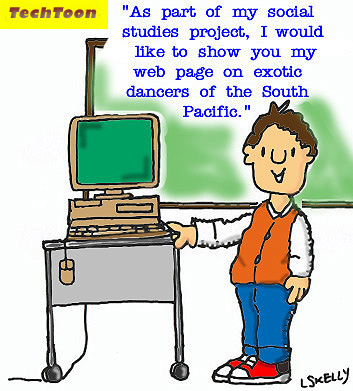
\includegraphics[width=0.60\textwidth]{figure/PublicProductDisasters.jpg}
	\caption{Public products require some careful thought -- Disaster projects might be range from  inaccurate and embarrassing and to useless and offensive (Yikes!). As the instructor, it is my role to provide the resources and guidance to help you develop projects we will be proud to make available to the public.}
	\label{fig:PublicProductDisasters}
\end{figure}

As you evaluate the pages to develop a set of standards and criteria that we can use to measure our own success.

\paragraph{Evaluation Criteria}

Each team will work to develop criteria that we can use to evaluate the public products, which will be further developed to evaluate each public product produced for our project.

\subsection{Session 2: How is the Earth's Temperature Taken?}

How are temperature data collected? This turns out to be a more complicated question that we might imagine at first. Let's begin by discussion what are the potential data quality issues with temperature data? We might begin by thinking about the data in terms of precision and accuracy.


that describes land-base Temperature data:

\begin{itemize}
  \item Land-based Temperatures
  %\item Sea-surface Temperatures
  %\item Remotely Sensed Data (e.g. Satellite) 
\end{itemize}

\subsubsection{Evaluation Criteria}

Evaluation criteria will be proposed by an "Expert Team" and inserted in Wiki. 

\subsection{Session 3: Where's [sic] the data!!!}

Watch this video

Use the Collaborative Documents to describe how weather is stored and made accessible. As part of this, we might need to better appreciate the sublties of how these data are stored, so we know our conclusions are reasonable.

\begin{enumerate*}
  \item How as data storage changed in the last 500 years?
  \item how data are curated? 
  \item how are data checked for quality?
\end{enumerate*}

\subsubsection{Evaluation Criteria}

How are the data store, curated and checked for quality?

\subsection{Session 4: Getting Data Effectively}

Let's begin by defining the characteristics of our data acqusition process. As a group please outline a series of criteria that should be used to ensure we can get data for our project. For example, we might consider getting data in reliable way. Or data that is updated regularly (e.g. daily, yearly).

Once you have defined the characteristics of the collecting process, I suggest you follow the next set of steps to acquire and prepare the data for the final product:

\begin{description}
  \item[Identify Data Sources] Each team will research and evaluate various sources of data. Create a Rmd file that describes the each data set, it sources and how it might become usuable using open sources of software. Develop scripts to download data (easier) or create a link to a database (preferrred). 
  \item[Pre-process data] Once the team has downloaded data, the files will need to be pre-processed to be imported into R and/or post-process to create a useful dataset. Large data set are often compressed using a vareity of protocols (e.g. zip, tar, gz). So, we we often have to "unzip", "untar", or "ungz". Once files are uncompressed, we need to look at the strcture of the files -- that might entail figuring how how columns have been separated or if there are long headers that might get in the way of the importing process. We will have to come up with various methods to deal with these data file strutures. 
  \item[Import data] requires a good understanding of the data structure and how a various software programs import data. We will use an open source software program called R.\footnote{Excel was not designed to handle large datasets, i.e. over ~1 million rows. For most purposes, this might be enough -- Many climate science data often exceed the number of observations that business programs like Excel was designed to do. However, even more compelling is that we are trying to create dataset that can be analyzed by anyone use a range of tools that are at our disposal as educated people. As such, I argue that we should be looking to open source. See the pdf on \href{https://rstudio.campus.pomona.edu/s/c2d027b9f6ba35ba4d250/files/github/Climate_Change_Narratives/Data/Liberation_via_Open_Source_Software.pdf}{Liberation through Open Source Software}.
} There are many resources to use R, including some handouts I have made. The functions to read files into R, include \texttt{read.csv()}, \texttt{read.table()}, etc. We will create some tools for us to use to make this process as painless as possible. 
  \item[Process data] Convert missing values to NA, naming variables, reshaping data);
\end{description}


\subsubsection{Evaluation Criteria for Session 5}

\subsection{Session X: Is there a case for Inference and Causation?}

  \begin{itemize*}
  		\item Artiola, J, Pepper, IL, Brusseau, M. 2004. Environmental Monitoring and Characterization. Chapter 3. Environmental Statistics (pp. 30-48).
\end{itemize*}

Each student will use a data source to create the public product where we can 
\begin{description}
  \item[Analyze] data for patterns (e.g. temporal trends); and
  \item[Create] compelling graphics (easier); or an interactive shiny app (perferred).
\end{description}


\section{Evaluating Narratives}

\subsection{Developing Criteria for Project Models}

\begin{itemize*}
  \item Team Work Contribution -- Did you fulfill the contract? Submit documentation that of your contribution to the team collaboration.
  \item Public Product
    \begin{itemize}
      \item Were the analysis methods and results described effectively?
    \end{itemize}

\end{itemize*}

\end{document}
